\section{Introduction}
Humans achieve effective natural language understanding by linking linguistic symbols 
to other modalities, e.g., vision, to establish a common ground where perceptual knowledge 
is generally shared. However, most prominent language representation pretraining frameworks 
like BERT and RoBERTa~\citep{devlin-etal-2019-bert,DBLP:journals/corr/abs-1907-11692} only 
take the language context in their self-supervision.

Recently, large-scale vision-language joint pretraining~(VLP) methods of learning 
cross-modal representation~\citep{lxmert,uniter,oscar} become increasingly popular for 
vision-language tasks, including visual question answering~\citep{vqa}, visual commonsense 
reasoning~\citep{vcr}, and image-text retrieval~\citep{itr}, etc. 

However, the performance of VLP methods were shown to exhibit notable declines when applied to pure-language tasks~\citep{voken}. There are two remarkable issues with
the previous methods:~(1) VLP methods learn linguistic representations from a specific type of language called \textit{grounded language}~\citep{groundedL1,groundedL2}, which has a large distributional disparity~(e.g., sentence length, vocabulary size, and n-gram distributions) with the other types of natural language. 
(2) The encoders for vision and text modalities in previous VLP methods are coupled 
(see \figref{fig:intro}). 
Consequently, if only textual inputs are given, such methods cannot effectively 
incorporate visual knowledge into their representations.
\begin{figure}[t]
	\centering
	\scalebox{1.0}{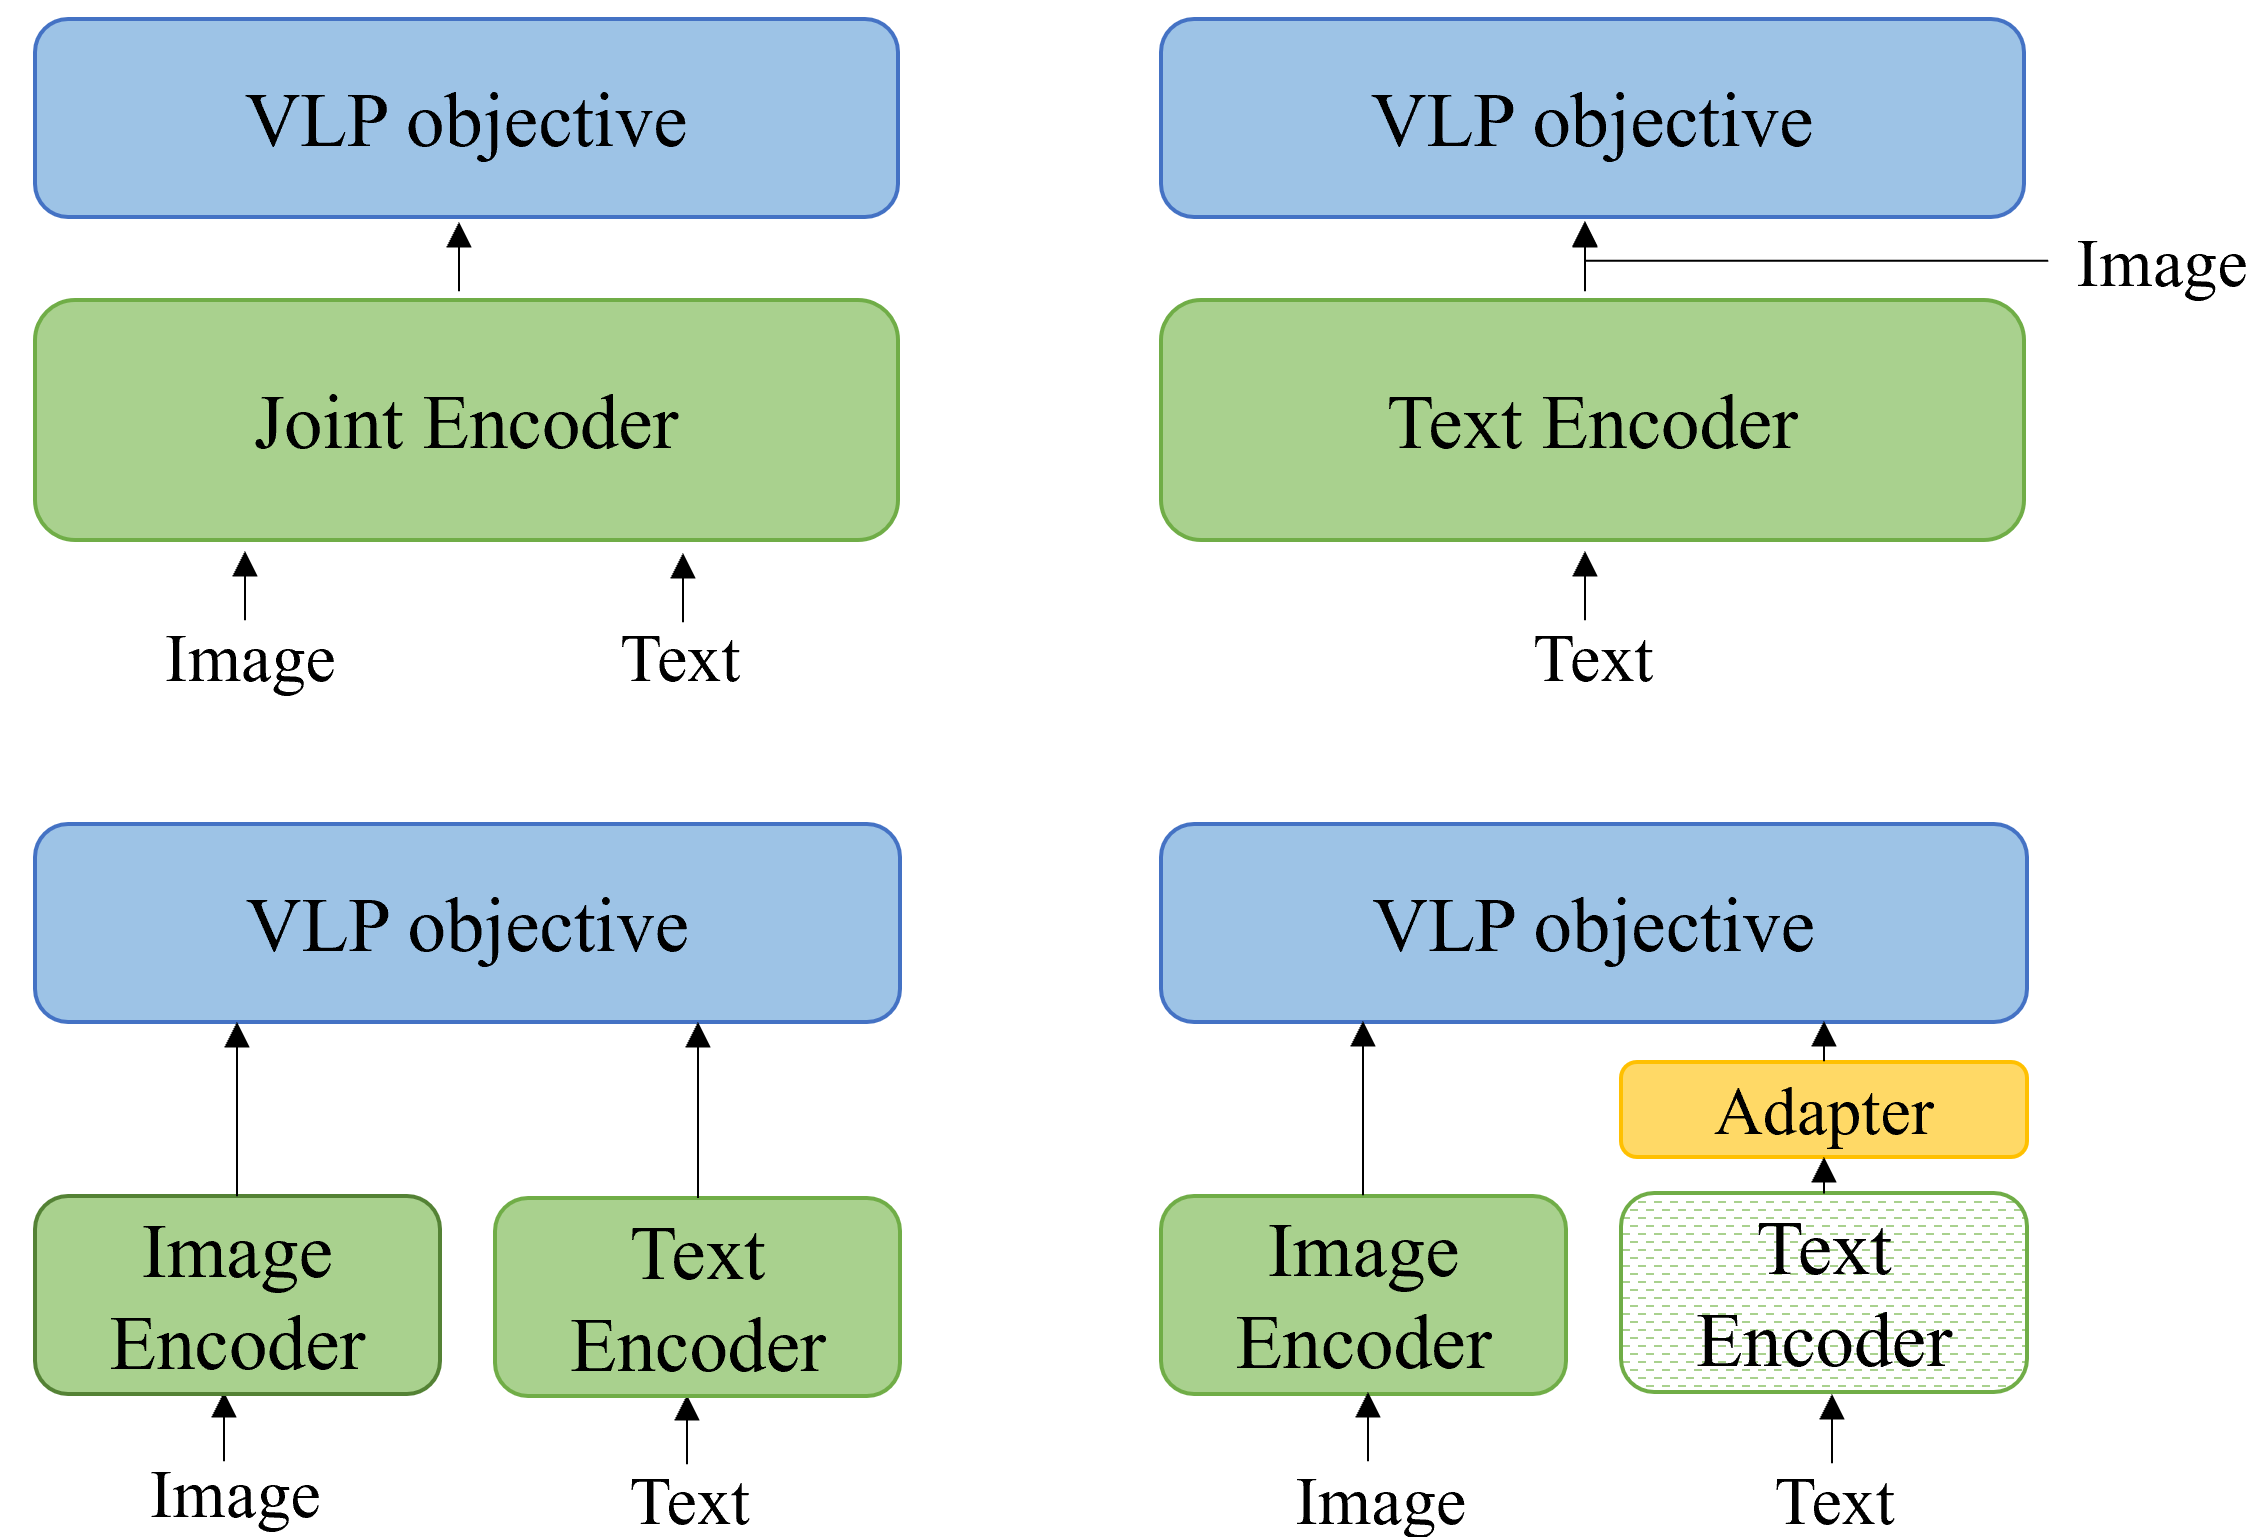
\includegraphics[width=1.0\columnwidth]{figures/intro_jq.png}}
	\caption{Schematic of four types of VLP paradigms: joint encoder~(top left), single text encoder~(top right), decoupled encoders~(bottom left), and our adapter-based encoder~(bottom right).} \label{fig:intro}
\end{figure} 
Accordingly, recent works have focused on improving VLP methods' performance on pure-language tasks by circumventing these two issues. \citet{voken} trained a contextual image retrieval model to create visual supervision for each token in large corpora, thereby bridging the gap between grounded language and other types of language. \citet{macd} proposed a multimodal decoupled learning framework, which forces the visual knowledge to be embedded in the text encoder. Though outperforming previous VLP methods on certain language understanding tasks, we show in experiment~(\secref{sec:main}) that they still suffer from deteriorated language representation capability and perform worse than the pretrained BERT.
\begin{figure*}[t!]
	\centering
	\scalebox{1.0}{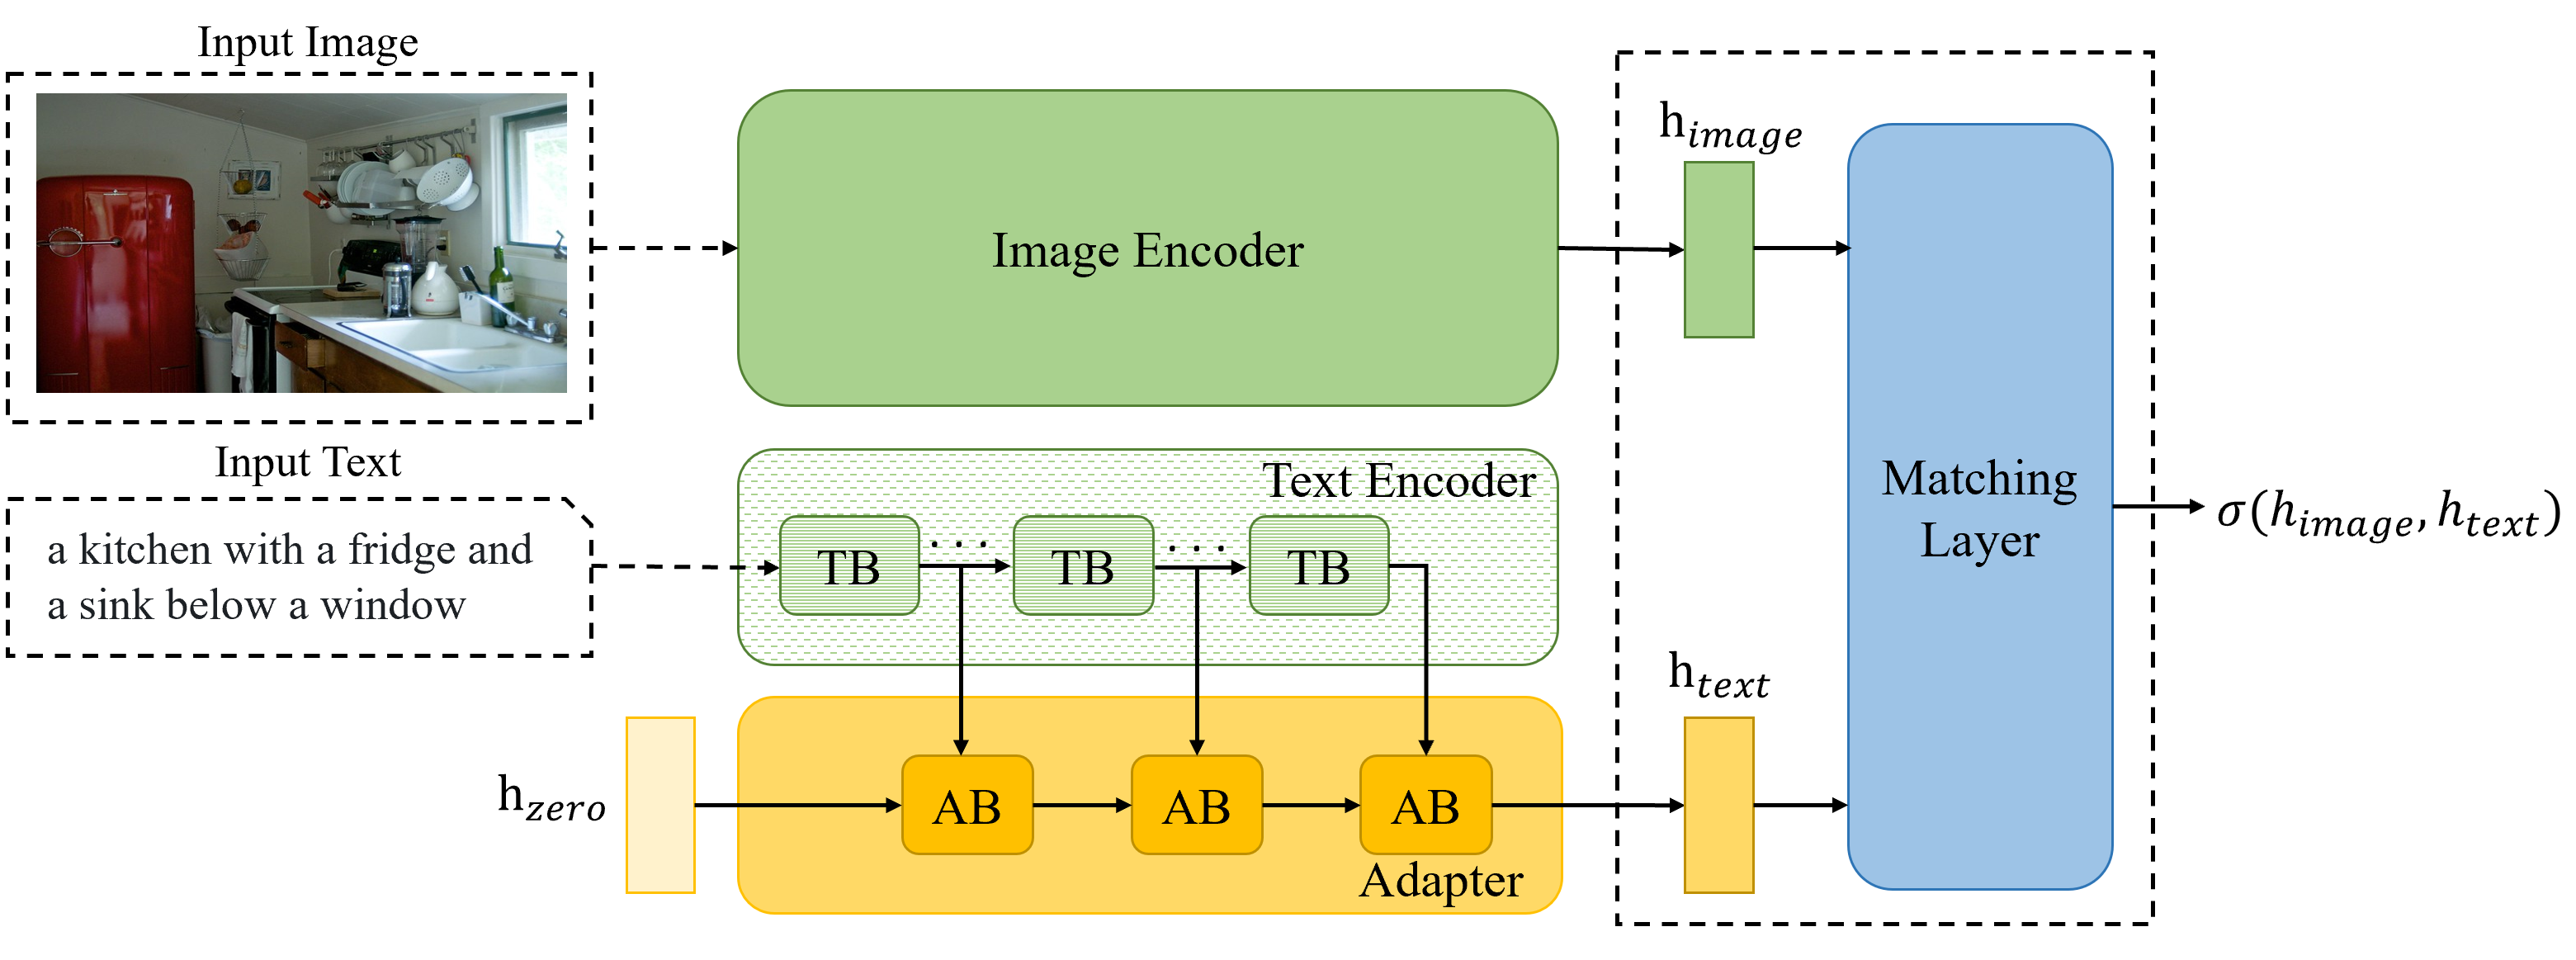
\includegraphics[width=2.0\columnwidth]{figures/overview.png}}
	\caption{Overall structure of our proposed Adapter-based Visual Grounding. TB stands for Transformer Block and AB stands for Adapter Block.} \label{fig:overview}
\end{figure*}

In this paper we investigate another approach, named \textbf{A}dapter-based \textbf{V}isual \textbf{G}rounding~(\textbf{AVG}), for reinforcing natural language understanding with visual knowledge. The schematic comparison between AVG and previous VLP methods is illustrated in \figref{fig:intro}. Specifically, instead of injecting visual knowledge directly into the text encoder, AVG extends previous decoupled encoder architecture by introducing a lightweight adapter module alongside the text encoder. The adapter takes as input pure-text representations produced by fixed text encoder and output refined representation that is encouraged to align with its corresponding image.


In experiment, we show that AVG enjoys two practical advantages over existing methods. 
First, AVG leaves the text encoder~(i.e., pretrained language model) unchanged and only 
update the adapter, thereby largely reducing memory footprint and facilitate training. Second, AVG delivers consistent improvements against other VLP baselines on several 
diverse understanding tasks by maximally retaining language modeling capability of the 
text encoder and adaptively leveraging visual knowledge learned during grounding. 
Case study using feature-based attribution method further reveals that AVG can better 
handle situations involving objects between which the relation can be generalized from 
multimodal grounding data.

We open-source code and pretrained adapters at: \url{https://anonymous.4open.science/r/r71s62ha12l312}.
